%%%%%%%%%%%%%%%%%%%%%%%%%%%%%%%%%%%%%%%%%
% Programming/Coding Assignment
% LaTeX Template
%
% This template has been downloaded from:
% http://www.latextemplates.com
%
% Original author:
% Ted Pavlic (http://www.tedpavlic.com)
%
% Note:
% The \lipsum[#] commands throughout this template generate dummy text
% to fill the template out. These commands should all be removed when 
% writing assignment content.
%
% This template uses a Perl script as an example snippet of code, most other
% languages are also usable. Configure them in the "CODE INCLUSION 
% CONFIGURATION" section.
%
%%%%%%%%%%%%%%%%%%%%%%%%%%%%%%%%%%%%%%%%%

%----------------------------------------------------------------------------------------
%	PACKAGES AND OTHER DOCUMENT CONFIGURATIONS
%----------------------------------------------------------------------------------------

\documentclass{article}

\usepackage{fancyhdr} % Required for custom headers
\usepackage{lastpage} % Required to determine the last page for the footer
\usepackage{extramarks} % Required for headers and footers
\usepackage[usenames,dvipsnames]{color} % Required for custom colors
\usepackage{graphicx} % Required to insert images
\usepackage{subcaption}
\usepackage{listings} % Required for insertion of code
\usepackage{courier} % Required for the courier font
\usepackage{lipsum} % Used for inserting dummy 'Lorem ipsum' text into the template

% Margins
\topmargin=-0.45in
\evensidemargin=0in
\oddsidemargin=0in
\textwidth=6.5in
\textheight=9.0in
\headsep=0.25in

\linespread{1.1} % Line spacing

% Set up the header and footer
\pagestyle{fancy}
\lhead{\hmwkAuthorName} % Top left header
\chead{\hmwkClass\ (\hmwkClassTime): \hmwkTitle} % Top center head
\rhead{\firstxmark} % Top right header
\lfoot{\lastxmark} % Bottom left footer
\cfoot{} % Bottom center footer
\rfoot{Page\ \thepage\ of\ \protect\pageref{LastPage}} % Bottom right footer
\renewcommand\headrulewidth{0.4pt} % Size of the header rule
\renewcommand\footrulewidth{0.4pt} % Size of the footer rule

\setlength\parindent{0pt} % Removes all indentation from paragraphs

%----------------------------------------------------------------------------------------
%	CODE INCLUSION CONFIGURATION
%----------------------------------------------------------------------------------------

\definecolor{MyDarkGreen}{rgb}{0.0,0.4,0.0} % This is the color used for comments
\lstloadlanguages{Perl} % Load Perl syntax for listings, for a list of other languages supported see: ftp://ftp.tex.ac.uk/tex-archive/macros/latex/contrib/listings/listings.pdf
\lstset{language=Perl, % Use Perl in this example
        frame=single, % Single frame around code
        basicstyle=\small\ttfamily, % Use small true type font
        keywordstyle=[1]\color{Blue}\bf, % Perl functions bold and blue
        keywordstyle=[2]\color{Purple}, % Perl function arguments purple
        keywordstyle=[3]\color{Blue}\underbar, % Custom functions underlined and blue
        identifierstyle=, % Nothing special about identifiers                                         
        commentstyle=\usefont{T1}{pcr}{m}{sl}\color{MyDarkGreen}\small, % Comments small dark green courier font
        stringstyle=\color{Purple}, % Strings are purple
        showstringspaces=false, % Don't put marks in string spaces
        tabsize=5, % 5 spaces per tab
        %
        % Put standard Perl functions not included in the default language here
        morekeywords={rand},
        %
        % Put Perl function parameters here
        morekeywords=[2]{on, off, interp},
        %
        % Put user defined functions here
        morekeywords=[3]{test},
       	%
        morecomment=[l][\color{Blue}]{...}, % Line continuation (...) like blue comment
        numbers=left, % Line numbers on left
        firstnumber=1, % Line numbers start with line 1
        numberstyle=\tiny\color{Blue}, % Line numbers are blue and small
        stepnumber=5 % Line numbers go in steps of 5
}

% Creates a new command to include a perl script, the first parameter is the filename of the script (without .pl), the second parameter is the caption
\newcommand{\perlscript}[2]{
\begin{itemize}
\item[]\lstinputlisting[caption=#2,label=#1]{#1.pl}
\end{itemize}
}

%----------------------------------------------------------------------------------------
%	DOCUMENT STRUCTURE COMMANDS
%	Skip this unless you know what you're doing
%----------------------------------------------------------------------------------------

% Header and footer for when a page split occurs within a problem environment
\newcommand{\enterProblemHeader}[1]{
\nobreak\extramarks{#1}{#1 continued on next page\ldots}\nobreak
\nobreak\extramarks{#1 (continued)}{#1 continued on next page\ldots}\nobreak
}

% Header and footer for when a page split occurs between problem environments
\newcommand{\exitProblemHeader}[1]{
\nobreak\extramarks{#1 (continued)}{#1 continued on next page\ldots}\nobreak
\nobreak\extramarks{#1}{}\nobreak
}

\setcounter{secnumdepth}{0} % Removes default section numbers
\newcounter{homeworkProblemCounter} % Creates a counter to keep track of the number of problems

\newcommand{\homeworkProblemName}{}
\newenvironment{homeworkProblem}[1][Problem \arabic{homeworkProblemCounter}]{ % Makes a new environment called homeworkProblem which takes 1 argument (custom name) but the default is "Problem #"
\stepcounter{homeworkProblemCounter} %Increase counter for number of problem
\renewcommand{\homeworkProblemName}{#1} % Assign \homeworkProblemName the name of the problem
\section{\homeworkProblemName} % Make a section in the document with the custom problem count
\enterProblemHeader{\homeworkProblemName} % Header and footer within the environment
}{
\exitProblemHeader{\homeworkProblemName} % Header and footer after the environment
}

\newcommand{\problemAnswer}[1]{ % Defines the problem answer command with the content as the only argument
\noindent\framebox[\columnwidth][c]{\begin{minipage}{0.98\columnwidth}#1\end{minipage}} % Makes the box around the problem answer and puts the content inside
}

\newcommand{\homeworkSectionName}{}
\newenvironment{homeworkSection}[1]{ % New environment for sections within homework problems, takes 1 argument - the name of the section
\renewcommand{\homeworkSectionName}{#1} % Assign \homeworkSectionName to the name of the section from the environment argument
\subsection{\homeworkSectionName} % Make a subsection with the custom name of the subsection
\enterProblemHeader{\homeworkProblemName\ [\homeworkSectionName]} % Header and footer within the environment
}{
\enterProblemHeader{\homeworkProblemName} % Header and footer after the environment
}

%----------------------------------------------------------------------------------------
%	NAME AND CLASS SECTION
%----------------------------------------------------------------------------------------

\newcommand{\hmwkTitle}{Assignment\ \#$\ 1$} % Assignment title
\newcommand{\hmwkDueDate}{Saturday,\ January\ 24,\ 2015} % Due date
\newcommand{\hmwkClass}{CSC320} % Course/class
\newcommand{\hmwkClassTime}{L0101} % Class/lecture time
\newcommand{\hmwkAuthorName}{Shihao Zhao} % Your name

%----------------------------------------------------------------------------------------
%	TITLE PAGE
%----------------------------------------------------------------------------------------

\title{
\vspace{2in}
\textmd{\textbf{\hmwkClass:\ \hmwkTitle}}\\
\normalsize\vspace{0.1in}\small{Due\ on\ \hmwkDueDate}\\
\vspace{0.1in}
\vspace{3in}
}

\author{\textbf{\hmwkAuthorName}}
%\date{} % Insert date here if you want it to appear below your name

%----------------------------------------------------------------------------------------

\begin{document}

\maketitle
\clearpage
%----------------------------------------------------------------------------------------
%	PART 0
%----------------------------------------------------------------------------------------

% To have just one problem per page, simply put a \clearpage after each problem

\begin{}

\noindent \textit{Part 0: Image data description}

The image data consists of three inverted negatives(top to bottom: blue, green, red). And in this project, we have small images and large images to work with. 
Here are some small and large images I worked with, Figure~\ref{fig:hat_man} - Figure~\ref{fig:train}.

%figure1
\begin{figure*}[h!]
    \centering
    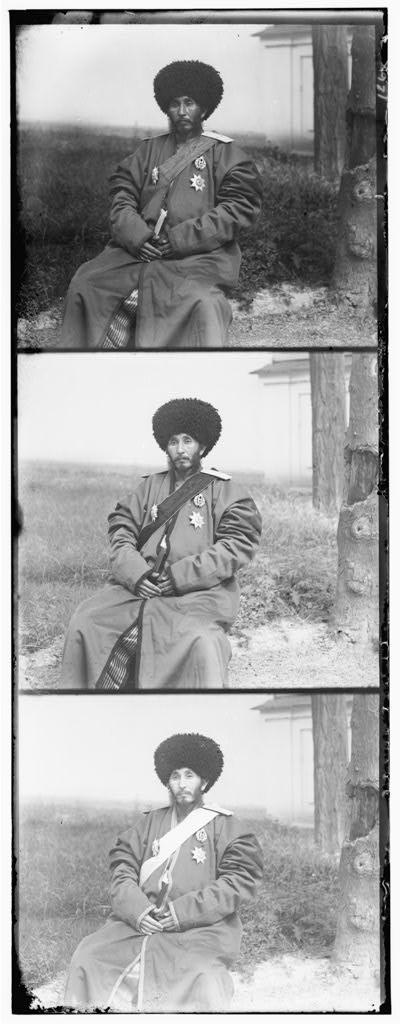
\includegraphics[scale=0.5]{00106v.jpg}
    \caption{This small image size is $1024 \times 401$.}
    \label{fig:hat_man}
\end{figure*}
%figure2
\begin{figure*}[h!]
    \centering
    \includegraphics[scale=0.5]{01880v.jpg}
    \caption{This small image size is $1024 \times 396$.}
    \label{fig:gate1}
\end{figure*}
%figure3
\begin{figure*}[h!]
    \centering
    \includegraphics[scale=0.5]{01031v.jpg}
    \caption{This small image size is $1024 \times 394$.}
    \label{fig:picture2}
\end{figure*}

%figure4
\begin{figure*}[h!]
    \centering
    \includegraphics[scale=0.5]{00128_shot1.png}
    \caption{This is a screen shot of the large image. The original image size is $9588 \times 3703$.}
    \label{fig:picture1}
\end{figure*}
%figure5
\begin{figure*}[h!]
    \centering
    \includegraphics[scale=0.5]{00458u_shot1.png}
    \caption{This is a screen shot of the large image. The original image size is $9715 \times 3741$.}
    \label{fig:train}
\end{figure*}

\end{homeworkProblem}
\clearpage
%----------------------------------------------------------------------------------------
%	PART 1
%----------------------------------------------------------------------------------------

\begin{}
\noindent \textit{Part 1: Comparing the matchings using SSD and NCC}

In this part, I will show three group of images, which will show the difference between the implementation of SSD and NCC. 


\begin{figure*}[h!]
    \centering
    \includegraphics[scale=0.5]{gate_SSD.png}
    \caption{This is the picture generated from 01880v.jpg using SSD. Generated using \texttt{A1('images/01880v.jpg', 0, 0)}.}
    \label{fig:25a}
\end{figure*}
\begin{figure*}[h!]
    \centering
    \includegraphics[scale=0.5]{gate_NCC.png}
    \caption{This one used NCC. Generated using 
\texttt{A1('images/01880v.jpg', 1, 0)}}
    \label{fig:mean_a}
\end{figure*}

These two work equally well as we can observe.
\clearpage

\begin{figure*}[h!]
    \centering
    \includegraphics[scale=0.5]{religion_SSD.png}
    \caption{This is the picture generated from 01031v.jpg using SSD. Generated using \texttt{A1('images/01031v.jpg', 0, 0)}.}
    \label{fig:religion_SSD}
\end{figure*}
\begin{figure*}[h!]
    \centering
    \includegraphics[scale=0.5]{religion_NCC.png}
    \caption{This one used NCC. Generated using 
\texttt{A1('images/01031v.jpg', 1, 0)}}
    \label{fig:religion_NCC}
\end{figure*}
These two have almost the same result, but if observing carefully, the NCC picture shows a little more details(see the characters in the pictures).
\clearpage

\begin{figure*}[h!]
    \centering
    \includegraphics[scale=0.5]{hat_SSD.png}
    \caption{This is the picture generated from 00106v.jpg using SSD. Generated using \texttt{A1('images/00106v.jpg', 0, 0)}.}
    \label{fig:hat_SSD}
\end{figure*}
\begin{figure*}[h!]
    \centering
    \includegraphics[scale=0.5]{hat_NCC.png}
    \caption{This one used NCC. Generated using 
\texttt{A1('images/00106v.jpg', 1, 0)}}
    \label{fig:hat_NCC}
\end{figure*}
This time, in my implementation, SSD works better. As we can observe in the NCC picture, the top edge on the man's hat turned green and the forehead of the man turned red. Overall, for most pictures, SSD and NCC works equally fine. But for the picture in which the contrast ratio is low, SSD will win. There are some artefacts in the result image. The noise on the border can impact it. The image where the colors of objects and background are similar can also impact it.

\end{homeworkProblem}
\clearpage
%----------------------------------------------------------------------------------------
%	PART 2
%----------------------------------------------------------------------------------------

\begin{}
\noindent \textit{Part 2: Results and runtime of large pictures}

In this part, I will show two groups of images, and describe the result and runtime.

\begin{figure*}[h!]
    \centering
    \includegraphics[scale=0.5]{picture_SSD.png}
    \caption{This is the combined picture from 00128u.png using SSD. Generated using \texttt{A1('images/00128u.png', 0, 1)}. The result picture has a decent quality, except for the noise on the border. However, the object in the picture is clear, and the edges of the object are recognizable. The running time of using SSD is roughly 12.4 sec on my computer(i7)}
    \label{fig:picture_SSD}
\end{figure*}
\begin{figure*}[h!]
    \centering
    \includegraphics[scale=0.5]{picture_NCC.png}
    \caption{This one used NCC. Generated using 
\texttt{A1('images/00128u.png', 1, 1)}. The quality result picture is okay, but not as good as SSD in my implementation. The edges of objects are kind of blurry.The running time is roughly 30 sec.}
    \label{fig:picture_NCC}
\end{figure*}

\textit{Advice: make observations about the output, and try to explain them.}
\clearpage

\begin{figure*}[h!]
    \centering
    \includegraphics[scale=0.5]{train_SSD.png}
    \caption{This is the combined picture from 00458u.png using SSD. Generated using \texttt{A1('images/00458u.png', 0, 1)}. The quality of result picture is good. The object in the picture is clear, and the edges of the object are recognizable. The running time of using SSD is roughly 11.7 sec on my computer(i7)}
    \label{fig:picture_SSD}
\end{figure*}
\begin{figure*}[h!]
    \centering
    \includegraphics[scale=0.5]{train_NCC.png}
    \caption{This one used NCC. Generated using 
\texttt{A1('images/00458u.png', 1, 1)}. The quality result picture is still not as good as SSD in my implementation. The edges of objects are kind of blurry.The running time is roughly 28 sec.}
    \label{fig:picture_NCC}
\end{figure*}
Overall, the running time is far longer than with small images, even though having used resizing algorithm. And the quality of result picture is good with SSD, but can be blurry with NCC in my implementation.
\textit{Advice: make observations about the output, and try to explain them.}

\end{homeworkProblem}
\clearpage


%----------------------------------------------------------------------------------------

\end{document}
